\documentclass{beamer}
\usepackage{amsmath, amsfonts, amssymb}

\usepackage{lmodern}
%\usepackage{sansmathaccent}
%\pdfmapfile{sansmathaccent.map}


\usepackage{graphicx}

\usepackage{multicol, multirow}

% We can use different themes 

% \usetheme {Warsaw}

\usetheme[progressbar = frametitle]{metropolis}
\setbeamertemplate {frame numbering}[fraction]
\useoutertheme {metropolis}
\useinnertheme{metropolis}
\usefonttheme{metropolis}
\usecolortheme{spruce}
\setbeamercolor{background canvas} {bg=white}



\definecolor{mygreen}{rgb}{.125, .5, .25}
\usecolortheme[named = mygreen ]{structure}

% \usecolortheme{crane}

% go to latexcolor.com to find out about more color theme. 

% Information regarding the title page (type 1) 
%\title[Future of Growth Perspective
%through Investment]{Future of Growth Perspective
%through Investment: \\ [2 pt]
%An Econometric Case Study of Bangladesh}
%\author{Chowdhury Amir Abdullah}
%\institute{University of Dhaka}
%\date{\today}


% Information regarding the title page (type 2) 
\title[Functions, Limits, Derivatives]{Functions, Limits, Derivatives}
%\subtitle{An Econometric Case Study of Bangladesh}
\author{}
\institute{\large \textbf{Learning Outcome}: \\ [6 pt] Identify properties of elementary functions (formed by composition of power, exponential, logarithmic, and trigonometric functions and their inverses.}
\date{}


\setbeamercovered{transparent =10}


\begin{document}

\metroset {block =fill}

% code for titlepage
\begin{frame}
\titlepage
\end{frame}



\begin{frame}[t]{Functions} \vspace{4 pt}

\begin{block} {Definition of a Function}
\vspace{0.5 em}
A \textbf{function} $f$ is a rule that assigns to each element $x$ in a set $D$ exactly one element, called $f(x)$ in a set $E$. 
\vspace{0.5 em}
\end{block}

\vspace{10 pt}

Set $D$ is called the 
\only<1>{ \line(1,0){50} }
\only<2> {\textcolor{magenta}{domain}}
\, of the function. \\ [10 pt]


Set $E$ is called the 
\only<1>{ \line(1,0){50} }
\only<2> {\textcolor{magenta}{range}}
\, of the function. 

\end{frame}





\begin{frame}{Your very first flash card} \vspace{10 pt}
\begin{columns}[onlytextwidth]
\column{0.4\textwidth}
$\sqrt{x^2}=$ \\ [10 pt]
\begin{enumerate}[(A)]
\item $x$
\item $-x$
\item $|x|$
\item undefined
\end{enumerate}
\column{0.6\textwidth}
\only<3>
{
$ 
\sqrt{x^2} =
\begin{cases}
-x, & x<0 \\
x, & x \geq 0
\end{cases}
$ \\[10pt]
}
\only<2->
{
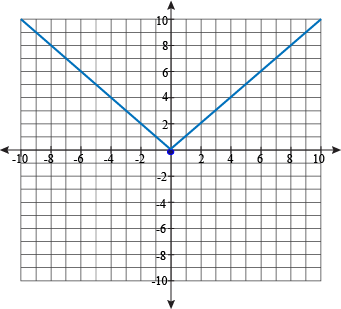
\includegraphics[scale=0.45]{squaredroot}
}
\end {columns}
\end{frame}






% \only command will remove the contents from your slide, so it might affect your alignment. 
% \onslide command just hides the contents, so it doesn't affect your alignment. 

\begin{frame}[t]{Parent Functions} \vspace{4pt} 
You should be able to identify by name and sketch a graph of each of the following parent functions.
\begin{enumerate}
\begin{multicols}{3}
\item $ y=x  $
\item $ y=|x| $
\item $ y=x^2 $
\item $ y=x^3 $
\item $ y=x^b $
\onslide<2->{
\item $ y=\sqrt{x} $
\item $ y=\sqrt[3]{x} $
\item $ y=\frac{1}{x} $
\item $ y=2^x $
\item $ y=e^x $}
\onslide<3->{
\item $ y=\ln x $
\item $ y=\frac{1}{1+e^{-x}} $
\item $ y=\sin x $
\item $ y=\cos x $
\item $ y=\tan x $}
\end{multicols}
\end{enumerate}
\end{frame}






\begin{frame}[standout]
\flushleft
Homework: p342, \# 7-23
\end{frame}

\end{document}